\documentclass[a4paper, 12pt]{article}
\usepackage[top=2cm, bottom=2cm, left=1cm, right=1cm]{geometry}
\usepackage{graphicx}
\usepackage{float}
\usepackage{booktabs}
\usepackage{pgfplots}
\usepackage{siunitx}

\begin{document}
	\begin{center}
		Universidade Federal do Rio Grande do Norte
		
		Departamento de Engenharia da Computação e Automação
		
		DCA3703 - Programação Paralela
		
		\textbf{Tarefa 3 - Aproximação matemática de $\pi$}
		
		\textbf{Aluno:} Daniel Bruno Trindade da Silva
	\end{center}
	
	\section{Introdução}
	
		\hspace{.6cm}Nesta tarefa, exploramos a aproximação de $\pi$ por meio de uma série matemática implementada em linguagem C. Foram realizadas variações no número de iterações do algoritmo, permitindo a análise da relação entre precisão e tempo de execução. Além disso, comparamos os valores obtidos com o valor real de $\pi$, avaliando a convergência da série e os impactos do aumento do processamento na acurácia dos resultados.
		
		
		Por fim, refletimos sobre a relevância desse comportamento em aplicações computacionais do mundo real, como simulações físicas e inteligência artificial, onde a necessidade de precisão influencia diretamente a eficiência e a confiabilidade dos resultados.
		
	\section{Metodologia}
		\hspace{.6cm}Para realizar a aproximação matemática de $\pi$ utilizaremos formula de Leibniz, que leva o nome de \textit{Gottfried Wilhelm Leibniz} um polímata alemão que viveu entre o século XVII e XVIII. A formula em notação de somatório é dada pelo seguinte:
		
		\begin{center}
			\[
			{\Huge \sum_{n=0}^{\infty} \frac{(-1)^n}{2n+1} = \frac{\pi}{4}}
			\]
		\end{center}
		
		Como se trata de uma série, quanto maior o valor de \textit{n}, mais aproximado do valor real de  $\pi$ será o valor que teremos como resultado. Para facilitar nosso trabalho implementamos uma função que possui um laço de repetição \texttt{for} que aplica a formula de Leibniz por \textit{n} vezes e a essa função demos o nome de  \texttt{piByLeibniz()} apos implementada ela ficou como se segue:
	
		\begin{verbatim}
			double piByLeibniz(int n) {
					double res_pi = 0.0;
					for (int i = 0; i < n; i++) {
							res_pi += ((i % 2 == 0) ? 1.0 : -1.0) / (2.0 * i + 1.0);
					}
					return 4.0 * res_pi;
			}
		\end{verbatim}
		
		Na \texttt{main()} de nosso código chamamos a função \texttt{piByLeibniz()} passando como parâmetro um valor de \textit{n} (que determina quantas iterações irão ocorrer para a aproximação). Essa função é chamada por \textit{x} vezes e a cada vez que é executada multiplica o valor de \textit{n} por 10. Logo na primeira chamada teremos o somatório de 10 termos, na segunda 100, na terceira 1000 e assim sucessivamente. Para nosso estudo realizaremos chamadas a função até \textit{n} assumir \( 10^{10} \), ou seja, teremos pi como o somatório de 10 bilhões de termos.
		
		A cada vez que chamarmos a função utilizaremos a \texttt{clock()} para medir o tempo convertendo os ticks para segundos, e assim saberemos quanto tempo cada chamada com um \textit{n} diferente vai levar. Em cada iteração exibimos o valor obtido para $\pi$ com 30 casas decimais, o tempo decorrido para o cálculo e o erro absoluto do valor em relação ao $\pi$ correto. Por fim nossa \texttt{main()} ficou da seguinte forma:
		
		\begin{verbatim}
			int main(){
					long long int n_it = 10;
					int num_test = 10;
					for(int i=0; i<num_test; i++){
							double pi, error;
							clock_t start = clock();
							pi = piByLeibniz(n_it);
							clock_t end = clock();
							printf("
									Valor obtido para pi: %.30f Tempo de execução com %lld iterações: %.4f ms\n",
									pi, n_it, get_time(start, end)
							);
							n_it *=10;
							error = fabs(M_PI - pi);
							printf("Erro absoluto: %.30f\n", error);
					}
				return 0;
			}
		\end{verbatim}
		
	\section{Resultados}
		\hspace{.6cm}A partir da saída do programa, podemos resgatar as informações que precisamos para analisar o desempenho obtido. Organizando os valores em uma tabela temos o seguinte:
		
		\begin{table}[h]
			\centering
			\small
			\begin{tabular}{r l l l}
				\toprule
				\textbf{Iterações} & \textbf{Valor de $\pi$} & \textbf{Erro absoluto} & \textbf{Tempo (ms)} \\
				\midrule
				10            & 3.041839618929403243896558706183   & 0.099753034660389872101404762361   & 0.0010  \\
				100           & 3.131592903558553686593768361490   & 0.009999750031239429404195107054   & 0.0000  \\
				1.000         & 3.140592653839794134995599961258   & 0.000999999749998981002363507287   & 0.0030  \\
				10.000        & 3.141492653590034489496929381858   & 0.000099999999758626501034086687   & 0.0220  \\
				100.000       & 3.141582653589719775766297971131   & 0.000010000000073340231665497413   & 0.3130  \\
				1.000.000     & 3.141591653589774324473182787187   & 0.000001000000018791524780681357   & 2.3300  \\
				10.000.000    & 3.141592553589791503299011310446   & 0.000000100000001612698952158098   & 22.3180 \\
				100.000.000   & 3.141592643589325994923910911893   & 0.000000010000467121074052556651   & 215.570 \\
				1.000.000.000 & 3.141592652588050427198140823748   & 0.000000001001742688799822644796   & 2155.49 \\
				10.000.000.000& 3.141592652878837377272702724440   & 0.000000000710955738725260744104   & 3026.95 \\
				\bottomrule
			\end{tabular}
			\caption{Resultados da aproximação de $\pi$ pela Série de Leibniz}
			\label{tab:pi_results}
		\end{table}
		
		Analisando a tabela podemos verificar que a convergência do valor obtido é muito custosa, foram necessárias 10 bilhões de iterações para conseguir chegar numa assertividade de 8 casas decimais. Isso pode ser visto mais claramente nos gráficos a seguir. 
		
		O primeiro deles mostra como o erro absoluto diminui en relação ao número de iterações confirmando o que já havíamos percebido na tabela a série de Leibniz converge para $\pi$, mas de forma lenta, exigindo um número muito grande de iterações para alcançar uma precisão aceitável. Em aplicações que exigem alta precisão, a utilização dessa série pode ser ineficiente, sendo necessário recorrer a métodos mais rápidos de convergência.
		
		\begin{figure}[H]
			\centering
			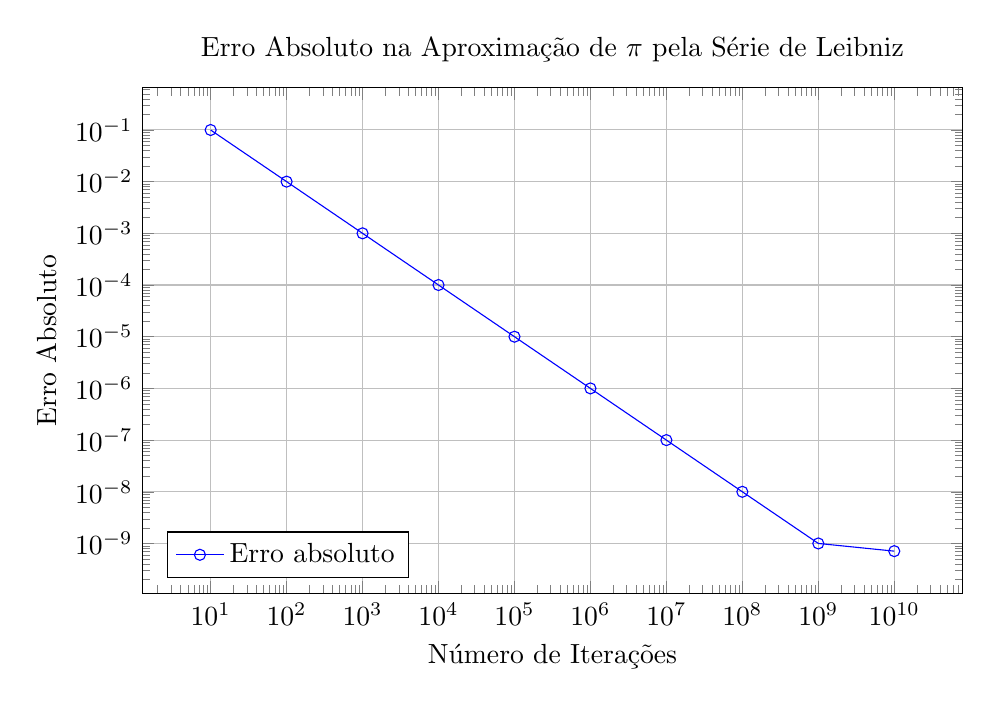
\begin{tikzpicture}
				\begin{loglogaxis}[
					width=12cm, height=8cm,
					xlabel={Número de Iterações},
					ylabel={Erro Absoluto},
					title={Erro Absoluto na Aproximação de $\pi$ pela Série de Leibniz},
					grid=major,
					legend pos=south west
					]
					\addplot[mark=o, color=blue] coordinates {
						(10, 0.099753034660389872101404762361)
						(100, 0.009999750031239429404195107054)
						(1000, 0.000999999749998981002363507287)
						(10000, 0.000099999999758626501034086687)
						(100000, 0.000010000000073340231665497413)
						(1000000, 0.000001000000018791524780681357)
						(10000000, 0.000000100000001612698952158098)
						(100000000, 0.000000010000467121074052556651)
						(1000000000, 0.000000001001742688799822644796)
						(10000000000, 0.000000000710955738725260744104)
					};
					\legend{Erro absoluto}
				\end{loglogaxis}
			\end{tikzpicture}
			\caption{Erro absoluto da aproximação de $\pi$ pela Série de Leibniz}
			\label{fig:erro_absoluto}
		\end{figure}
		
		No segundo gráfico vemos o custo em tempo por número de iterações. Podemos observar um crescimento exponencial do tempo de execução conforme o número de iterações aumenta, evidenciando o custo computacional da aproximação. Esse comportamento reforça a necessidade de um equilíbrio entre precisão e eficiência computacional, especialmente em aplicações que exigem cálculos rápidos e precisos.
		
		
		\begin{figure}[H]
			\centering
			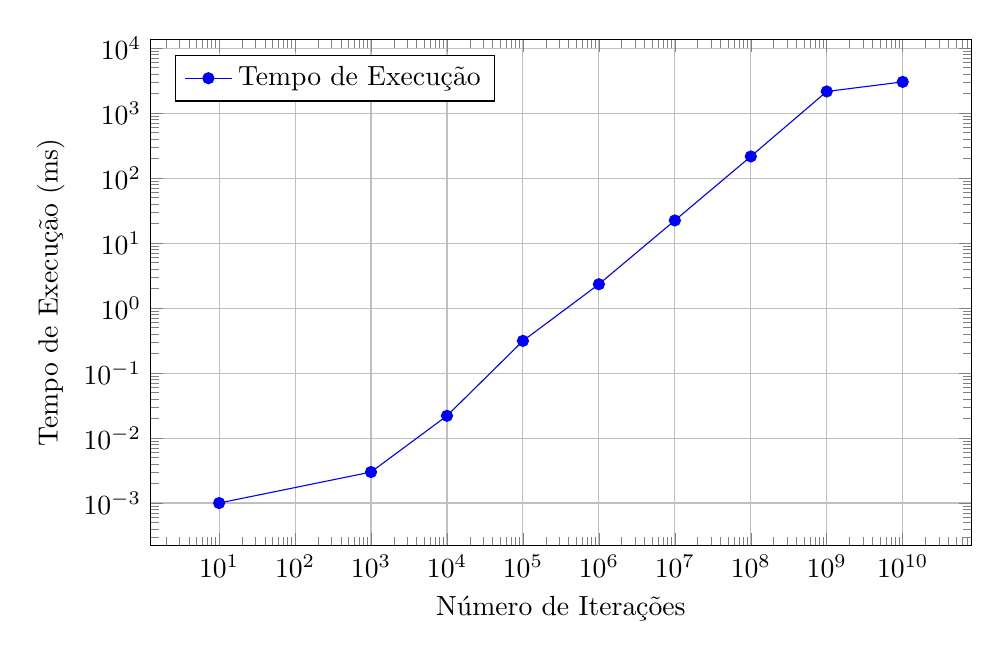
\begin{tikzpicture}
				\begin{axis}[
					xlabel={Número de Iterações},
					ylabel={Tempo de Execução (ms)},
					xmode=log,
					log basis x=10,
					ymode=log,
					log basis y=10,
					grid=major, % Grade nas linhas principais
					width=12cm, height=8cm, % Define o tamanho do gráfico
					legend pos=north west % Posição da legenda
					]
					\addplot[color=blue, mark=*] coordinates {
						(10, 0.0010)
						(100, 0.0000)
						(1000, 0.0030)
						(10000, 0.0220)
						(100000, 0.3130)
						(1000000, 2.3300)
						(10000000, 22.3180)
						(100000000, 215.570)
						(1000000000, 2155.49)
						(10000000000, 3026.95)
					};
					\addlegendentry{Tempo de Execução}
				\end{axis}
			\end{tikzpicture}
			\caption{Crescimento do tempo de execução com o aumento do numero de iterações}
		\end{figure}
		
	\section{Conclusão}
	\hspace{.6cm}A relação observada entre precisão e tempo de execução na aproximação de $\pi$ pela Série de Leibniz reflete um desafio comum em diversas aplicações computacionais do mundo real. Em áreas como simulações físicas e inteligência artificial, a necessidade de obter resultados cada vez mais precisos frequentemente exige maior poder computacional, o que pode impactar o tempo de processamento e o consumo de recursos.
	
	Por exemplo, em simulações físicas, como as utilizadas em modelagem climática ou dinâmica de fluidos, pequenas imprecisões nos cálculos podem levar a grandes desvios nos resultados finais. Métodos numéricos de alta precisão são essenciais, mas, assim como no caso da Série de Leibniz, a busca por maior acurácia pode aumentar exponencialmente o tempo de processamento. Por isso, técnicas como refinamento adaptativo de malhas e algoritmos de alta eficiência são frequentemente adotadas para otimizar esse balanço entre precisão e desempenho.
	
	Na inteligência artificial, especialmente no treinamento de redes neurais profundas, um dilema semelhante ocorre. Modelos mais complexos e precisos geralmente demandam maior capacidade computacional e tempo de treinamento. No entanto, técnicas como quantização de modelos, uso de aproximações matemáticas eficientes e treinamento distribuído ajudam a mitigar esses desafios, permitindo que modelos de IA sejam treinados e executados de maneira mais eficiente sem perder significativamente a precisão.
	
	Portanto, o comportamento observado no experimento com a Série de Leibniz evidencia um princípio fundamental da computação: quanto maior a precisão desejada, maior o custo computacional associado. Esse dilema exige que se busquem métodos alternativos que equilibrem precisão e eficiência, tornando os cálculos viáveis para aplicações práticas no mundo real.
		
	
\end{document}